\documentclass[twoside]{article}
\usepackage{graphicx}
\usepackage{amsmath}
\usepackage{amssymb}
\usepackage{booktabs}
\usepackage{blindtext}
\usepackage{changepage}
\usepackage{setspace}
\usepackage{parskip}
\usepackage[margin=1in]{geometry}
\usepackage{microtype}
\usepackage{listings}
\usepackage{xcolor}
\usepackage{enumitem}
\usepackage{hyperref}

\colorlet{punct}{red!60!black}
\definecolor{background}{HTML}{EEEEEE}
\definecolor{delim}{RGB}{20,105,176}
\colorlet{numb}{magenta!60!black}

\lstdefinelanguage{json}{
    basicstyle=\ttfamily\small,
    numbers=left,
    numberstyle=\tiny\color{gray},
    stepnumber=1,
    numbersep=8pt,
    showstringspaces=false,
    breaklines=true,
    frame=single,
    backgroundcolor=\color{background},
    literate=
     *{0}{{{\color{numb}0}}}{1}
      {1}{{{\color{numb}1}}}{1}
      {2}{{{\color{numb}2}}}{1}
      {3}{{{\color{numb}3}}}{1}
      {4}{{{\color{numb}4}}}{1}
      {5}{{{\color{numb}5}}}{1}
      {6}{{{\color{numb}6}}}{1}
      {7}{{{\color{numb}7}}}{1}
      {8}{{{\color{numb}8}}}{1}
      {9}{{{\color{numb}9}}}{1}
      {:}{{{\color{punct}{:}}}}{1}
      {,}{{{\color{punct}{,}}}}{1}
      {\{}{{{\color{delim}{\{}}}}{1}
      {\}}{{{\color{delim}{\}}}}}{1}
      {[}{{{\color{delim}{[}}}}{1}
      {]}{{{\color{delim}{]}}}}{1},
}

\lstset{
    basicstyle=\ttfamily\small,
    breaklines=true,
    frame=single,
    backgroundcolor=\color{background},
    keywordstyle=\color{blue},
    stringstyle=\color{red},
    commentstyle=\color{green!50!black},
    numbers=left,
    numberstyle=\tiny\color{gray},
    captionpos=b
}
\setlist[itemize]{leftmargin=1.5em}
\setlist[enumerate]{leftmargin=1.5em}

\begin{document}

\setlength{\parskip}{10pt plus 2pt minus 2pt}
\setlength{\parindent}{15pt}

%\fancyfoot{}
%\renewcommand{\footrulewidth}{0pt}

\title{COMP Workshop KBQA System Design Report}
%\shorttitle{My Template}
%\leadauthor{Author}

% Use letters for affiliations, numbers to show equal authorship (if applicable) and to indicate the corresponding author
\author{Author}

\maketitle

\setlength{\parskip}{10pt plus 2pt minus 2pt}
\setlength{\parindent}{15pt}

\section{Introduction}

The proposed RAG framework integrates hybrid retrieval with reranking-enhanced generation to optimize answer accuracy. The principal workflow is shown as Figure~\ref{fig:pipeline}. The following content introduces our pipeline briefly.

\section{Workflow of the KBQA System}

\begin{itemize}
    \item \textbf{Hybrid Retrieval Mechanism}
    \begin{itemize}
        \item \textit{Keyword Model}: Utilizes BM25/TF-IDF for lexical matching, calculating keyword relevance scores based on term frequency patterns.
        \item \textit{Semantic Model}: Employs text-embedding models (e.g., BAAI/bge-m3) to compute semantic similarity scores via cosine similarity.
        \item \textit{Hybrid Fusion}: Combines keyword and semantic scores through weighted averaging, balancing lexical and semantic signals.
    \end{itemize}
    
    \item \textbf{Context-Aware Reranking}
    \begin{itemize}
        \item Processes top 20 hybrid-ranked documents using BERT-style BAAI/bge-reranker-v2-m3 model~\cite{reranker:chen2024airbenchautomatedheterogeneousinformation} for query-context interaction analysis.
        \item Implements dynamic relevance refinement through attention mechanisms.
    \end{itemize}
    
    \item \textbf{Generation Pipeline}
    \begin{itemize}
        \item Leverages Qwen2.5-7B-Instruct with structured prompting:
        \begin{itemize}
            \item Priority weighting for retrieved contexts via template engineering.
            \item Fallback protocols triggering ``I don't know'' responses for irrelevant content.
        \end{itemize}
    \end{itemize}
\end{itemize}

\begin{figure}[htbp]
  \centering
  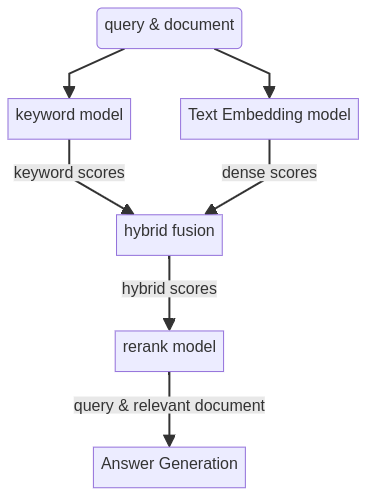
\includegraphics[width=.8\linewidth]{Figures/flowchart.png}
  \caption{Flowchart diagram of our pipeline.}
  \label{fig:pipeline}
  \end{figure}

We apply some enhancement techniques including document chunk optimization (sliding windows, pooling scores), hybrid retrieval with sparse+dense method, prompt engineering.

\section{Method}

\subsection{Keyword Matching-Based Retrieval}
In our question-answering system, we experimented with \textbf{TF-IDF}, \textbf{BM25}, and a simple hybrid of the two. These two methods are widely used in information retrieval to quantify the importance of a term within a document relative to a collection of documents. We implemented TF-IDF and BM25 using the \texttt{scikit-learn} and \texttt{rank\_bm25} libraries, respectively.

\paragraph*{TF-IDF}

TF-IDF (Term Frequency-Inverse Document Frequency) computes the importance of a term $t$ in document $d$ within a corpus $D$ using the following formula:

\[
\text{TF-IDF}(t, d, D) = \text{TF}(t, d) \cdot \text{IDF}(t, D)
\]

where:
\[
\text{TF}(t, d) = f_{t,d}, \quad \text{IDF}(t, D) = \log \left( \frac{1 + N}{1 + n_t} \right) + 1
\]

Here, $f_{t,d}$ is the frequency of term $t$ in document $d$, $N$ is the total number of documents, and $n_t$ is the number of documents containing term $t$. The additive smoothing (``+1'') prevents division by zero.

\paragraph*{BM25}

BM25 is a probabilistic ranking function that enhances TF-IDF by introducing document length normalization and term frequency saturation. The BM25 score of term $t$ in document $d$ is given by:

\[
\text{BM25}(t, d) = \text{IDF}(t) \cdot \frac{f_{t,d} \cdot (k_1 + 1)}{f_{t,d} + k_1 \cdot (1 - b + b \cdot \frac{|d|}{\text{avgdl}})}
\]

where:
\[
\text{IDF}(t) = \log \left( \frac{N - n_t + 0.5}{n_t + 0.5} + 1 \right)
\]

Here, $f_{t,d}$ is the frequency of term $t$ in document $d$, $|d|$ is the length of document $d$, $\text{avgdl}$ is the average document length in the corpus, and $k_1$, $b$ are tunable hyperparameters (typically $k_1 = 1.5$, $b = 0.75$). This formulation prevents long documents from being unfairly favored and moderates the influence of very high term frequencies.

\medskip




\subsection{Dense Embedding Model-Based Retrieval}

In this part, this project fine-tunes the pre-trained language encoding model to generate dense embeddings for both documents and queries.
We use these embeddings to calculate the similarity between documents and queries. Considering the BERT-base-uncased model has a token limit
of 512, which is far shorter than the tokenization length of most documents. Therefore, we choose to fine-tune Nomic-BERT-2048 for better 
performance in long documents. Inspired by the Dense Passage Retrieval (DPR) model, we design a two-tower structure to map queries and
documents independently into the same semantic space, enabling efficient semantic matching. The two-tower structure not only improves 
retrieval speed but also significantly enhances the accuracy of semantic matching, providing high-quality results for downstream tasks.

\paragraph*{The construction of fine-tuned dataset}

We need to build supervised learning data samples, which include query text (questions), positive documents (text containing answers), and 
negative documents (text without answers). Although most documents still exceed the model's input limits after tokenization, models that 
support long tokens can capture semantic information more accurately. The Nomic-BERT-2048 model supports 2048 token inputs and offers 
advantages such as preserving complete semantic units, reducing information fragmentation, and providing richer context. Leveraging these 
features, we designed a smart chunking strategy~\cite{fama2024no} to ensure that both positive and negative samples retain complete semantic information.
For short documents, we keep them intact without chunking to preserve their semantic structure and context, avoiding unnecessary semantic 
loss from splitting. For long documents, we use an overlapping sliding window approach to chunk them, maintaining an overlap area 
(default 100 words) between adjacent chunks to ensure contextual coherence and prevent key information from being split. We also maximize 
the chunk size (default 1800 words) to fully utilize Nomic BERT 2048's long-sequence capability, reducing the number of chunks significantly 
compared to traditional BERT models. Additionally, each chunk retains full metadata, including the source document ID, original position, 
and chunk sequence number, for easy processing and traceability. Through this strategy, we support long document processing while ensuring 
semantic integrity and retrieval efficiency.

\begin{figure}[htbp]
    \centering
    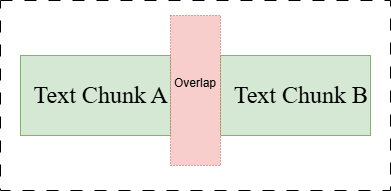
\includegraphics[width=0.5\textwidth]{Figures/chunk_op.png}
    \caption{The diagram shows the overlapping relationship between 
    two text chunks. In the figure, two bright green rectangles 
    represent ``Text Chunk A'' and ``Text Chunk B''. They are connected 
    by a pink rectangle labeled ``Overlap'', which shows the shared 
    content between the two adjacent text segments.}
    \label{fig:chunk-overlap}
\end{figure}
To build positive samples, we combine exact matching and overlap assessment. First, we filter chunks in the target document that contain the 
answer text, ensuring positive samples have the answer. If multiple chunks contain the answer, we pick the most relevant one by calculating the 
answer's coverage proportion in each chunk, aiming to get the most complete answer context. Thanks to processing large text chunks, positive samples 
usually include the full answer context for richer semantics.

Negative sample quality is key for the model's ability to distinguish. We use three types: random docs unrelated to the question, positive samples 
of other questions in the same batch, and hard negative samples~\cite{doringer2023synthetic} that are semantically related to the question but lack the answer. 
Hard negative samples are the most challenging but best for improving the model's distinction ability.

To find hard negative samples, we use a TF-IDF similarity-based strategy. First, we convert the question text into a TF-IDF vector to capture key 
semantic features. Then, we calculate the cosine similarity between the question vector and all document chunk vectors to get semantic relevance scores. 
Next, we rank document chunks by similarity in descending order and select those meeting the criteria, excluding chunks from the same source as the 
question's associated document and chunks with answer text. Finally, we pick multiple (default 3) semantically relevant negative samples for each 
question to boost training diversity.

\begin{figure}[htbp]
\centering
\begin{lstlisting}[language=json]
{
"question": "who plays erwin ...",
"pos_ctx": "The film stars ...",
"neg_ctxs": [
"Europe throughout the ...",
"I Still Haven't Found What ...",
"Samsung Galaxy Note Edge..."
]
}
\end{lstlisting}
\caption{Training data JSON structure example (content simplified)}
\label{fig:dpr-json}
\end{figure}

Simply speaking, we split text into chunks like pieces of a jigsaw puzzle. Text chunks with known answers are like the correct puzzle pieces and 
serve as positive training samples, teaching the model to recognize semantically similar content. Text chunks with similar keywords but no answers 
are like puzzle pieces that seem to fit but are misplaced; these are hard negative samples that make training more challenging. We also add unrelated 
and random negative samples, akin to puzzle pieces that clearly don't belong to the picture, to help the model fine-tune its ability to distinguish 
truly relevant content. Through this mix, the model not only learns to spot correct answers but also stays accurate amid distractions, improving its ability 
to find right answers in complex contexts.

\paragraph*{Dual-tower architecture and vector representation learning}

The core of the DPR model lies in its dual-tower architecture, which consists of two separate encoders: a query encoder and a document encoder. Both encoders 
are based on the Nomic BERT 2048 pre-trained model, but they are optimized for different objectives in text representation. The query encoder focuses on capturing the 
core semantics and intent of a question, while the document encoder emphasizes extracting key information from long texts. During training, we align the vector spaces 
of the two encoders through contrastive learning to achieve semantic matching. The representation of the CLS token is normalized using L2 normalization and used as the 
final vector, making it easier for subsequent similarity calculations. Training the DPR model requires careful tuning of a series of hyperparameters to adapt to the 
characteristics of long text processing and contrastive learning. The key configurations we use include: a learning rate of 3e-5, the AdamW optimizer (with epsilon=1e-08), 
5 training epochs, a batch size of 4, and gradient accumulation steps of 2. The whole training is done in the NVIDIA GeForce RTX 2080Ti 22G GPU. These parameters 
have been optimized through repeated experiments to ensure training stability while fully leveraging the long-text understanding capabilities of Nomic-BERT-2048. 
The setting of the temperature parameter (0.05) is critical for the model to distinguish between positive and negative samples, as a lower temperature value helps the model 
form a clearer decision boundary.
\subsection{Hybrid Retrieval}

To leverage both lexical and semantic information, we employ a hybrid retrieval approach~\cite{langchain2023hybrid} that combines keyword-based and semantic-based scores through weighted averaging. Specifically, for a given query \( q \) and document \( d \), the hybrid score is calculated as:

\[ s_{\text{hybrid}}(q, d) = \alpha \cdot s_{\text{keyword}}(q, d) + (1 - \alpha) \cdot s_{\text{semantic}}(q, d) \]

where:
\begin{itemize}
    \item \( s_{\text{keyword}}(q, d) \) is the keyword-based relevance score, obtained from a combination of BM25 and TF-IDF methods.
    \item \( s_{\text{semantic}}(q, d) \) is the semantic similarity score, computed using cosine similarity between the query and document embeddings.
    \item \( \alpha \in [0, 1] \) is a weighting parameter that balances the contribution of keyword and semantic scores.
\end{itemize}

The keyword score \( s_{\text{keyword}}(q, d) \) is itself a weighted combination of BM25 and TF-IDF scores:

\[ s_{\text{keyword}}(q, d) = \beta \cdot s_{\text{BM25}}(q, d) + (1 - \beta) \cdot s_{\text{TF-IDF}}(q, d) \]

where \( \beta \in [0, 1] \) is the weight for BM25. In our experiments, we found that \( \beta = 0.7 \) yields the best performance for the keyword component, as evidenced by the results in the Experiments section.

The semantic score \( s_{\text{semantic}}(q, d) \) is computed using pre-trained text-embedding models, such as BAAI/bge-m3, which generate dense vector representations for the query and documents. The cosine similarity is then calculated as:

\[ s_{\text{semantic}}(q, d) = \frac{\mathbf{e}_q \cdot \mathbf{e}_d}{\|\mathbf{e}_q\| \|\mathbf{e}_d\|} \]

where \( \mathbf{e}_q \) and \( \mathbf{e}_d \) are the embedding vectors of the query and document, respectively.

By adjusting the parameter \( \alpha \), we can control the influence of lexical versus semantic matching in the retrieval process. This hybrid approach allows us to capture both exact keyword matches and deeper semantic relationships between the query and documents.

\subsection{Rerank Retrieval}

To further refine the ranking of the retrieved documents, we incorporate a reranking step using the BAAI/bge-reranker-v2-m3 model. This model is a transformer-based reranker that evaluates the relevance of each document to the query by considering their pairwise interactions.

Specifically, after obtaining the top 20 documents based on the hybrid retrieval scores, we pass each query-document pair through the reranker to compute a more precise relevance score. The reranker model outputs a score \( s_{\text{rerank}}(q, d) \) for each pair, which is used to re-rank the documents.

The final ranking of the documents is determined by sorting them in descending order of their reranker scores. This step enhances the retrieval quality by leveraging the model's ability to capture complex semantic relationships and contextual relevance that may not be fully captured by the initial hybrid scores.

Mathematically, the reranking process can be described as follows:

\begin{enumerate}
    \item Select the top \( k = 20 \) documents based on the hybrid scores \( s_{\text{hybrid}}(q, d) \).
    \item For each of these top \( k \) documents, compute the reranker score \( s_{\text{rerank}}(q, d) \) using the BAAI/bge-reranker-v2-m3 model.
    \item Re-rank the documents based on \( s_{\text{rerank}}(q, d) \) in descending order.
\end{enumerate}


\subsection{Pre-trained DPR Model-Based Retrieval}
In this part, we use the pre-trained DPR model to generate dense embeddings for both documents and queries. We want to use these embeddings to improve 
the performance of the KBQA system.

\paragraph*{The pre-trained DPR model BAAI/bge-m3}

BAAI/bge-m3 is an open-source embedding model developed by the Beijing Academy of Artificial Intelligence (BAAI). It is designed for information retrieval (IR) applications 
and is known for its versatility in multi-functionality, multi-linguality, and multi-granularity. The model supports over 100 languages and can handle semantic matching tasks 
across different languages.

BGE-M3 generates semantic vectors using the CLS token, making it suitable for semantic matching tasks. It can process inputs ranging from short sentences to long documents of 
up to 8192 tokens, handling text at various granularities such as ``sentences,'' ``paragraphs,'' ``chapters,'' and ``documents.'' A single inference can produce outputs in multiple modes 
without additional overhead, efficiently supporting hybrid retrieval. Combining three retrieval modes (dense, sparse, and multi-vector) yields more accurate retrieval results.

BAAI/bge-m3 excels in tasks like multi-lingual and cross-lingual retrieval, as well as long document search. It is applicable in various scenarios such as semantic search, keyword 
search, and re-ranking. As a powerful embedding model, it meets diverse information retrieval needs, particularly excelling in multi-lingual and long-text processing.

\paragraph*{Deep semantic embedding for long document retrieval}
Even though the bge-m3 model supports a token limit of up to 8192, some documents in real-world applications are still much longer than this limit. To handle these extra-long documents 
effectively, we used a chunking strategy. When splitting the documents into chunks, we kept a 20\% overlap between adjacent chunks to ensure semantic coherence. After processing each chunk, 
we applied weighted average pooling, where the weights were based on the length of each chunk, to generate the final dense vectors for retrieval. We applied this method to both queries and 
documents and stored the generated vectors in a FAISS vector database to speed up retrieval.

In simple terms, longer document chunks naturally contain more information and context. To reflect this, we apply a weighted approach based on the length of each chunk. This way, longer chunks 
contribute more to the final semantic vector, giving them greater semantic weight and enhancing the accuracy and expressiveness of the representation. By doing this, we ensure the semantic vector 
better captures the overall meaning of the document, improving both retrieval efficiency and effectiveness.

\begin{figure}[htbp]
  \centering
  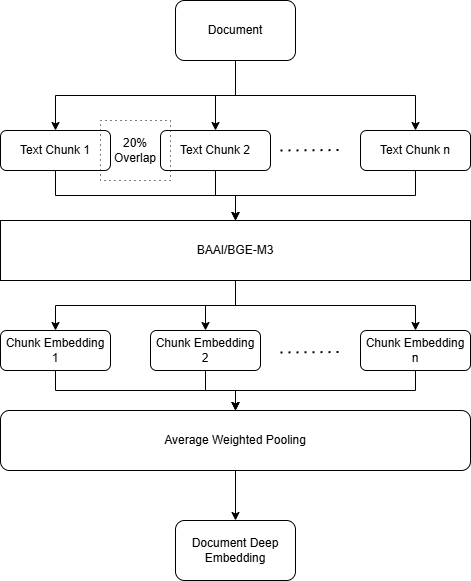
\includegraphics[width=0.5\textwidth]{Figures/bgem3.png}
  \caption{The diagram shows the process of document deep embedding. First, the document is divided into several text chunks, with a 20\% overlap between each chunk. These text chunks are then processed 
  by the BAAI/BGE-M3 model to generate corresponding chunk embeddings. Next, an average weighted pooling method is used to integrate all the chunk embeddings, resulting in the document's deep embedding 
  representation.}
  \label{fig:bgem3}
\end{figure}

Through evaluation, this method achieved a Document Retrieval Recall@5 of 0.9070 and a Document Retrieval MRR@5 of 0.7405, showing that it works well for document retrieval tasks and effectively
improves retrieval efficiency and accuracy.

\subsection{Answer Generation}
\paragraph*{Prompt}
In the generation phase of our Retrieval-Augmented Generation (RAG) framework, we utilize a structured prompt to guide the language model, Qwen2.5-7B-Instruct~\cite{qwen25model}, in producing accurate and contextually relevant answers. This prompt is designed to ensure that the model adheres strictly to the retrieved context, minimizing the risk of generating extraneous or incorrect information. It employs XML-like tags to delineate the context and query, coupled with explicit instructions to enforce precise and concise responses. The prompt template is shown below:

\begin{figure}[htbp]
\centering
\begin{lstlisting}[language=xml]
<context>{context}</context>
<query>{query}</query>

Instructions:
1. query is wrapped in <query></query> 
   tags
2. context is wrapped in <context>
   </context> tags
3. Answer the query based strictly 
   on the content
4. If the answer cannot be found in 
   <context>, return <answer>wrong
   </answer>
5. Valid answers must:
   - Be wrapped in <answer></answer> 
     tags
   - Contain only key terms/phrases
   - Maintain concise reliability
6. Format: <answer>your answer</answer>
\end{lstlisting}
\caption{Prompt template for the Qwen2.5-7B-Instruct model.}
\end{figure}

\vspace{0.5cm}

This structured prompting approach enhances the model's ability to generate reliable answers by clearly defining the input structure and output expectations, aligning with our pipeline's emphasis on context-aware generation.

% %%%%%%%%%%%%%%Experiments%%%%%%%%%%%%%%%5
\section{Experiment}
\subsection{Keyword Retrieval experiment}

We evaluated the effectiveness of keyword-based retrieval using a weighted hybrid of \textbf{BM25} and \textbf{TF-IDF} on preprocessed documents. Specifically, we tested different linear combinations of BM25 and TF-IDF scores to determine the optimal weighting for document ranking. The text preprocessing methods are detailed in the supplementary materials. 

\vspace{5pt}
\begin{table}[htbp]
\centering
\setlength{\tabcolsep}{10pt}
\begin{tabular}{p{3cm} c c}
\toprule
\textbf{BM25 / TF-IDF Weight} & \textbf{Recall@5} & \textbf{MRR@5} \\
\midrule
{1.0 / 0.0}               & 0.7210 & 0.5728 \\
{0.8 / 0.2}                 & 0.7930 & 0.6339 \\
\textbf{0.7 / 0.3}                 & \textbf{0.8020} & \textbf{0.6283} \\
0.5 / 0.5                          & 0.7850 & 0.6006 \\
0.3 / 0.7                          & 0.7370 & 0.5544 \\
0.0 / 1.0                          & 0.6930 & 0.5128 \\
\bottomrule
\end{tabular}
\caption{Retrieval Performance with Different BM25/TF-IDF Weights}
\end{table}
\vspace{5pt}

\paragraph*{Experiment Conclusion}
As expected, BM25 outperformed TF-IDF. However, both methods performed worse on their own compared to their weighted combination. This result highlights the advantage of hybrid keyword matching. The best retrieval performance was achieved by combining scores with a weighting of \textbf{0.7 BM25 + 0.3 TF-IDF}.
% %%%%%%%%%%%%%%%%%%%%%%%%%%%%%%%5
\subsection{Benchmarks}

\vspace{5pt}
\begin{table}[htbp]
\centering
\setlength{\tabcolsep}{10pt}
\begin{tabular}{p{3cm} c c}
\toprule
\textbf{Retrieval Method} & \textbf{Recall@5} & \textbf{MRR@5} \\
\midrule
keyword & 0.7850 & 0.6006 \\
keyword+rerank & 0.8700 & 0.7254 \\
dense & 0.9070 & 0.7405 \\
dense+rerank & 0.9080 & 0.7555 \\
\bottomrule
\end{tabular}
\caption{Retrieval Performance Comparison of Different Methods}
\label{tab:dataset_metrics}
\end{table}
\vspace{5pt}


% %%%%%%%%%%%%%%%%%%%%%%%%%%%%%%%%

\section{Interface UI Design}
This system adopts a Retrieval-Augmented Generation (RAG) architecture, with the WebUI module serving as the frontend interface for the entire question-answering system, responsible for user interaction and functionality visualization. The system workflow is divided into five stages: user query reception, document retrieval, retrieval result reranking, answer generation, and result presentation.

The WebUI is built on the Gradio framework, adopting an object-oriented design pattern. It primarily consists of the WebUI class as the core component, as well as the create\_webui helper function for creating and launching WebUI instances.

The entire system workflow can be divided into the following stages:

\begin{enumerate}
    \item User query reception: Receiving user questions through the WebUI
    \item Document retrieval: Using various retrieval methods to find relevant documents from the document library
    \item Document reranking: Reranking the retrieval results to improve relevance
    \item Answer generation: Generating answers using large language models based on the retrieved documents
    \item Result presentation: Displaying the generated answers and relevant documents to the user
\end{enumerate}

The Web UI system architecture is illustrated as follows:

\begin{figure}[htbp]
  \centering
  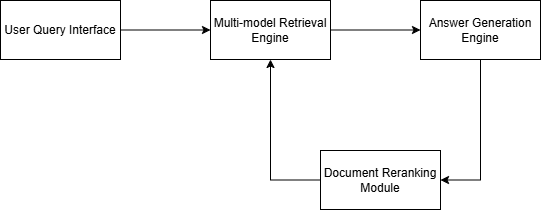
\includegraphics[width=0.5\textwidth]{Figures/UI.png}
  \caption{The diagram shows the architecture which demonstrates the interaction flow between the key components of the system: the user query interface handles user input, the multi-modal retrieval engine searches for relevant documents, the document reranking module improves search result quality, and the answer generation engine produces the final response.}
  \label{fig:ui}
\end{figure}

\subsection{WebUI Class}
The WebUI class is the core of the interface, responsible for initializing retrievers, building the interface, and processing user queries. It includes the following functional groups:

\begin{itemize}
    \item Configuration management: Loading system configurations through ``load\_config'' methods
    \item Retrieval functionality: Providing three retrieval approaches - traditional retrieval based on BM25, semantic retrieval based on DPR, and hybrid retrieval
    \item Ranking and generation: Reranking retrieval results through ``rerank\_results'' and generating final answers using ``generate\_answer''
    \item Query processing: The ``process\_query'' method serves as the coordinator of the core processing flow
    \item Interface construction: The ``build\_ui'' and ``launch'' methods are responsible for building and launching the Gradio interface
\end{itemize}

\subsection{Retrieval Module}
The system supports three retrieval strategies, fully leveraging the advantages of both traditional methods and deep learning:

\begin{itemize}
    \item ``BM25'' retrieval: A classic algorithm based on term frequency and inverse document frequency, handling exact matches
    \item ``DPR'' retrieval: Using the ``BGE-M3'' model to generate semantic vectors, with efficient retrieval through ``FAISS''
    \item ``Hybrid retrieval'': Combining the strengths of the previous two methods, first obtaining candidate documents, then optimizing results through reranking
\end{itemize}

\subsection{Reranking and Generation Modules}
The reranking module uses the ``ReRanker'' class, based on the BGE-reranker model, to perform fine-grained ranking of retrieval results, improving relevance. The answer generation module utilizes ``QwenChatClient'' to call the Qwen model, generating high-quality answers through carefully designed prompt engineering and a strategy of multiple generations to select the optimal result.

\subsection{Technical Features}
\paragraph*{Asynchronous Processing Mechanism}
The system extensively adopts ``asyncio'' to implement asynchronous processing, including asynchronous API requests, multi-threaded service startup, and asynchronous batch processing, effectively enhancing system concurrency and responsiveness.

\paragraph*{Optimized Answer Generation Strategy}
The system implements an innovative answer generation strategy: when one document cannot provide an effective answer, it automatically attempts the next relevant document. Simultaneously, it generates multiple answers for the same question and selects the most likely result through a voting mechanism, significantly improving the accuracy and reliability of answers.

\paragraph*{Flexible Configuration Management}
The system manages various parameters through ``YAML'' configuration files, including ``WebUI'' settings, retrieval method parameters, model configurations, etc., providing a high degree of customization to meet the needs of different scenarios.

\paragraph*{User Interaction Design}

\bibliographystyle{plain}
\bibliography{zHenriquesLab-Mendeley}

\end{document}
